% !TeX root = ../main-paper.tex
\section{Results}

\subsection{OCR evaluation}

\begin{figure}

\subcaptionbox{}[.5\linewidth]{
\begin{tabular}{rll}
          & CER & CER$_{norm.}$ \\
\midrule
Pero      & 3.78\% & 3.76\% \\   
Tesseract & 6.56\% & 6.45\% \\
\bottomrule
\end{tabular}

\bigskip

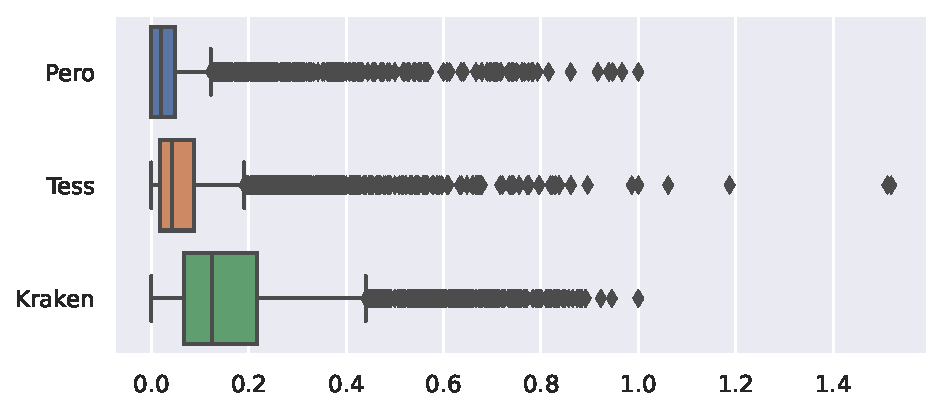
\includegraphics[width=\linewidth]{images/ocr-eval-2.pdf}
}
\subcaptionbox{}[.5\linewidth]{
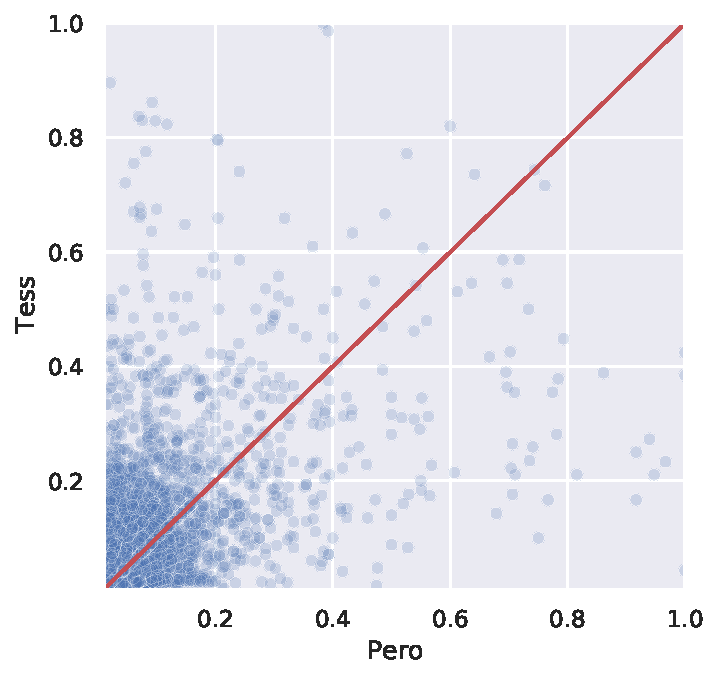
\includegraphics[width=\linewidth]{images/ocr-eval-1.pdf}
}
\caption{Character error rates at entry-level for Pero OCR and Tesseract. (a) Global CER and distribution of the CER per entry. (b):
joint plot of the dataset showing that the two systems do not fail on the same entries.}  
\end{figure}

\subsection{Experiment 1: NER sensibility to the number of training samples}

Qualitative results
\textbf{TODO random samples of results + selection of failure cases}


Quantitative results: table + graph ideally (with training set size info)

\begin{table}[h!]
\centering
\caption{NER performances at entry-level for SpaCy NER, CamemBERT and CamemBERT-pretrained when fine-tuned with an increasing number of examples.}
\begin{tabular}{llrrrrrrrr}
       & Training examples &  49   &  99   &  199  &  398  &  796  &  1593 &  3186 &  6373 \\
       & \% & 0.8   & 1.6   & 3.1   & 6.2   & 12.5  & 25.0  & 50.0  & 100.0 \\
\midrule\bottomrule
\multirow{3}{*}{\rotatebox{90}{F1 score}} & Camembert &  89.5 &  90.5 &  92.7 &  93.3 &  \textbf{94.1} &  \textbf{94.9} &  \textbf{94.6} &  \textbf{95.1} \\
       & Camembert-pretrained &  \textbf{92.2} &  \textbf{92.9} &  \textbf{93.6} &  \textbf{93.8} &  93.8 &  94.1 &  \textbf{94.6} &  94.4 \\
       & SpaCy NER &  87.0 &  89.0 &  90.3 &  91.9 &  92.1 &  92.8 &  93.2 &  93.5 \\
\cline{1-10}
\multirow{3}{*}{\rotatebox{90}{Precision}} & Camembert &  87.4 &  88.7 &  91.5 &  92.7 &  93.3 &  94.9 &  93.9 &  95.1 \\
       & Camembert-pretrained &  90.8 &  91.8 &  92.9 &  93.0 &  93.0 &  93.4 &  94.1 &  93.9 \\
       & SpaCy NER &  85.6 &  87.7 &  90.0 &  92.0 &  92.4 &  92.8 &  93.1 &  93.7 \\
\cline{1-10}
\multirow{3}{*}{\rotatebox{90}{Recall}} & Camembert &  91.6 &  92.5 &  93.9 &  93.9 &  94.9 &  94.9 &  95.4 &  95.1 \\
       & Camembert-pretrained &  93.6 &  94.0 &  94.4 &  94.6 &  94.6 &  94.8 &  95.0 &  94.9 \\
       & SpaCy NER &  88.6 &  90.4 &  90.7 &  91.7 &  91.9 &  92.8 &  93.3 &  93.4 \\
\end{tabular}
\label{tab:experiment-1-models-performances}
\end{table}


\begin{figure}[h!]
	   \center{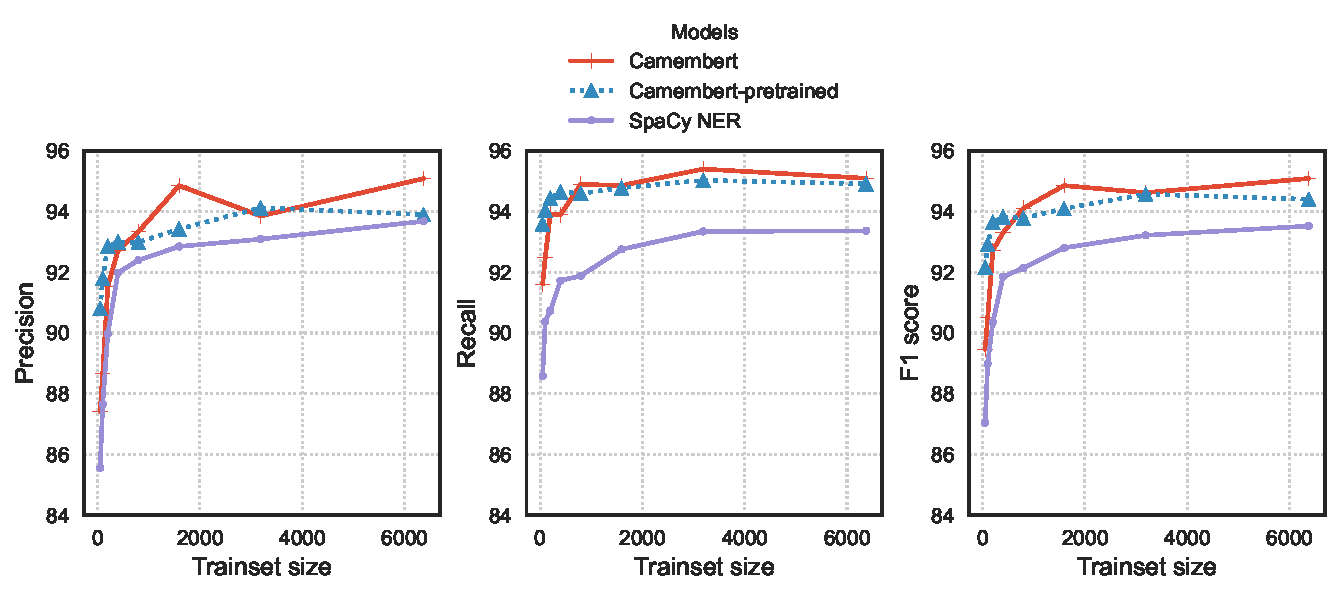
\includegraphics[width=\textwidth]
	       {images/experiment-1-models-performances.pdf}}
	  \caption{\label{fig:f1-vs-trainsize} Precision, recall and f1 score from table~\ref{tab:experiment-1-models-performances}}.
\end{figure}
	                                        


\subsection{Experiment 2: NER in the presence of noisy OCR texts}

Qualitative results
\textbf{TODO random samples of results + selection of failure cases}

Quantitative results: table + graph ideally (with OCR noise, same format as previous)

Table : NER NN models VS train on {noisy, clean} datasets VS evaluate on {noisy, clean} datasets

\begin{figure}
    \centering
    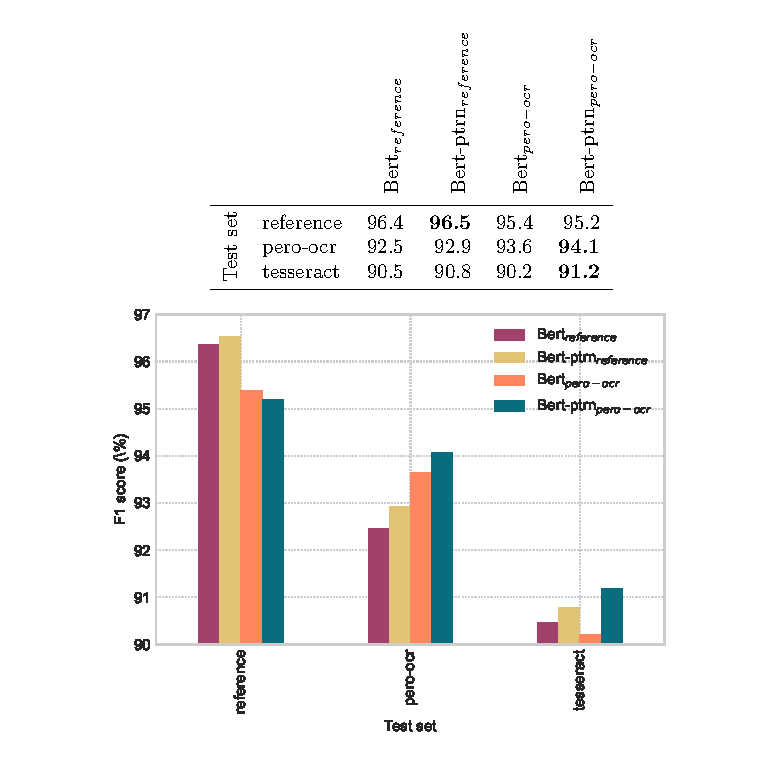
\includegraphics[width=\textwidth]{figs/eval-ner-exp2.pdf}
    \caption{F1 scores (in \%) of NER predictions in presence of OCR noise in the training and testing examples, either manually corrected or raw from Pero-OCR and Tesseract. The type of examples used to train the NER task is noted in indice after the model name (e.g. Bert$_{reference}$). Results show that best performances on OCRed entries are obtained when the BERT model has been pretrained and fine-tuned for NER on examples affected with similar OCR errors.}
    \label{fig:exp_2_eval_ner}
\end{figure}
Opt. use synthetic text perturbation as well? Maybe not interesting and too artificial if we have access to 2+ OCR systems.
(original OCR from BNF, Tesseract 4, Pero OCR…)


\subsection{Discussion}
Interesting points to discuss:
\begin{itemize}
    \item can we train on noisy data? (without manual OCR correction?) => future work? cf Pero OCR training procedure?
    \item do we need better OCR systems or better post-correction techniques (if NER is reliable enough)?
    \item Construction of the lexicon and associated cost
\end{itemize}
